\documentclass[twoside]{book}

% Packages required by doxygen
\usepackage{calc}
\usepackage{doxygen}
\usepackage{graphicx}
\usepackage[utf8]{inputenc}
\usepackage{makeidx}
\usepackage{multicol}
\usepackage{multirow}
\usepackage{textcomp}
\usepackage[table]{xcolor}

% Font selection
\usepackage[T1]{fontenc}
\usepackage{mathptmx}
\usepackage[scaled=.90]{helvet}
\usepackage{courier}
\usepackage{amssymb}
\usepackage{sectsty}
\renewcommand{\familydefault}{\sfdefault}
\allsectionsfont{%
  \fontseries{bc}\selectfont%
  \color{darkgray}%
}
\renewcommand{\DoxyLabelFont}{%
  \fontseries{bc}\selectfont%
  \color{darkgray}%
}

% Page & text layout
\usepackage{geometry}
\geometry{%
  a4paper,%
  top=2.5cm,%
  bottom=2.5cm,%
  left=2.5cm,%
  right=2.5cm%
}
\tolerance=750
\hfuzz=15pt
\hbadness=750
\setlength{\emergencystretch}{15pt}
\setlength{\parindent}{0cm}
\setlength{\parskip}{0.2cm}
\makeatletter
\renewcommand{\paragraph}{%
  \@startsection{paragraph}{4}{0ex}{-1.0ex}{1.0ex}{%
    \normalfont\normalsize\bfseries\SS@parafont%
  }%
}
\renewcommand{\subparagraph}{%
  \@startsection{subparagraph}{5}{0ex}{-1.0ex}{1.0ex}{%
    \normalfont\normalsize\bfseries\SS@subparafont%
  }%
}
\makeatother

% Headers & footers
\usepackage{fancyhdr}
\pagestyle{fancyplain}
\fancyhead[LE]{\fancyplain{}{\bfseries\thepage}}
\fancyhead[CE]{\fancyplain{}{}}
\fancyhead[RE]{\fancyplain{}{\bfseries\leftmark}}
\fancyhead[LO]{\fancyplain{}{\bfseries\rightmark}}
\fancyhead[CO]{\fancyplain{}{}}
\fancyhead[RO]{\fancyplain{}{\bfseries\thepage}}
\fancyfoot[LE]{\fancyplain{}{}}
\fancyfoot[CE]{\fancyplain{}{}}
\fancyfoot[RE]{\fancyplain{}{\bfseries\scriptsize Generated on Wed Apr 22 2015 22\-:34\-:19 for My Project by Doxygen }}
\fancyfoot[LO]{\fancyplain{}{\bfseries\scriptsize Generated on Wed Apr 22 2015 22\-:34\-:19 for My Project by Doxygen }}
\fancyfoot[CO]{\fancyplain{}{}}
\fancyfoot[RO]{\fancyplain{}{}}
\renewcommand{\footrulewidth}{0.4pt}
\renewcommand{\chaptermark}[1]{%
  \markboth{#1}{}%
}
\renewcommand{\sectionmark}[1]{%
  \markright{\thesection\ #1}%
}

% Indices & bibliography
\usepackage{natbib}
\usepackage[titles]{tocloft}
\setcounter{tocdepth}{3}
\setcounter{secnumdepth}{5}
\makeindex

% Hyperlinks (required, but should be loaded last)
\usepackage{ifpdf}
\ifpdf
  \usepackage[pdftex,pagebackref=true]{hyperref}
\else
  \usepackage[ps2pdf,pagebackref=true]{hyperref}
\fi
\hypersetup{%
  colorlinks=true,%
  linkcolor=blue,%
  citecolor=blue,%
  unicode%
}

% Custom commands
\newcommand{\clearemptydoublepage}{%
  \newpage{\pagestyle{empty}\cleardoublepage}%
}


%===== C O N T E N T S =====

\begin{document}

% Titlepage & ToC
\hypersetup{pageanchor=false}
\pagenumbering{roman}
\begin{titlepage}
\vspace*{7cm}
\begin{center}%
{\Large My Project }\\
\vspace*{1cm}
{\large Generated by Doxygen 1.8.6}\\
\vspace*{0.5cm}
{\small Wed Apr 22 2015 22:34:19}\\
\end{center}
\end{titlepage}
\clearemptydoublepage
\tableofcontents
\clearemptydoublepage
\pagenumbering{arabic}
\hypersetup{pageanchor=true}

%--- Begin generated contents ---
\chapter{Hierarchical Index}
\section{Class Hierarchy}
This inheritance list is sorted roughly, but not completely, alphabetically\-:\begin{DoxyCompactList}
\item Mono\-Behaviour\begin{DoxyCompactList}
\item \contentsline{section}{Bomb\-Script}{\pageref{classBombScript}}{}
\item \contentsline{section}{Bullets}{\pageref{classBullets}}{}
\item \contentsline{section}{Destroy\-By\-Time}{\pageref{classDestroyByTime}}{}
\item \contentsline{section}{Game\-Camera}{\pageref{classGameCamera}}{}
\item \contentsline{section}{Game\-Controller}{\pageref{classGameController}}{}
\item \contentsline{section}{Game\-Manager}{\pageref{classGameManager}}{}
\item \contentsline{section}{Health}{\pageref{classHealth}}{}
\begin{DoxyCompactList}
\item \contentsline{section}{Player\-Controller}{\pageref{classPlayerController}}{}
\end{DoxyCompactList}
\item \contentsline{section}{Med\-Pack}{\pageref{classMedPack}}{}
\item \contentsline{section}{Object\-Behavior2}{\pageref{classObjectBehavior2}}{}
\item \contentsline{section}{Player\-Physics}{\pageref{classPlayerPhysics}}{}
\item \contentsline{section}{Spike\-Obstacle}{\pageref{classSpikeObstacle}}{}
\item \contentsline{section}{Test\-Colliderand\-Health}{\pageref{classTestColliderandHealth}}{}
\end{DoxyCompactList}
\end{DoxyCompactList}

\chapter{Class Index}
\section{Class List}
Here are the classes, structs, unions and interfaces with brief descriptions\-:\begin{DoxyCompactList}
\item\contentsline{section}{\hyperlink{classBombScript}{Bomb\-Script} }{\pageref{classBombScript}}{}
\item\contentsline{section}{\hyperlink{classBullets}{Bullets} }{\pageref{classBullets}}{}
\item\contentsline{section}{\hyperlink{classDestroyByTime}{Destroy\-By\-Time} }{\pageref{classDestroyByTime}}{}
\item\contentsline{section}{\hyperlink{classGameCamera}{Game\-Camera} }{\pageref{classGameCamera}}{}
\item\contentsline{section}{\hyperlink{classGameController}{Game\-Controller} }{\pageref{classGameController}}{}
\item\contentsline{section}{\hyperlink{classGameManager}{Game\-Manager} }{\pageref{classGameManager}}{}
\item\contentsline{section}{\hyperlink{classHealth}{Health} }{\pageref{classHealth}}{}
\item\contentsline{section}{\hyperlink{classMedPack}{Med\-Pack} }{\pageref{classMedPack}}{}
\item\contentsline{section}{\hyperlink{classObjectBehavior2}{Object\-Behavior2} }{\pageref{classObjectBehavior2}}{}
\item\contentsline{section}{\hyperlink{classPlayerController}{Player\-Controller} }{\pageref{classPlayerController}}{}
\item\contentsline{section}{\hyperlink{classPlayerPhysics}{Player\-Physics} }{\pageref{classPlayerPhysics}}{}
\item\contentsline{section}{\hyperlink{classSpikeObstacle}{Spike\-Obstacle} }{\pageref{classSpikeObstacle}}{}
\item\contentsline{section}{\hyperlink{classTestColliderandHealth}{Test\-Colliderand\-Health} }{\pageref{classTestColliderandHealth}}{}
\end{DoxyCompactList}

\chapter{Class Documentation}
\hypertarget{classBombScript}{\section{Bomb\-Script Class Reference}
\label{classBombScript}\index{Bomb\-Script@{Bomb\-Script}}
}
Inheritance diagram for Bomb\-Script\-:\begin{figure}[H]
\begin{center}
\leavevmode
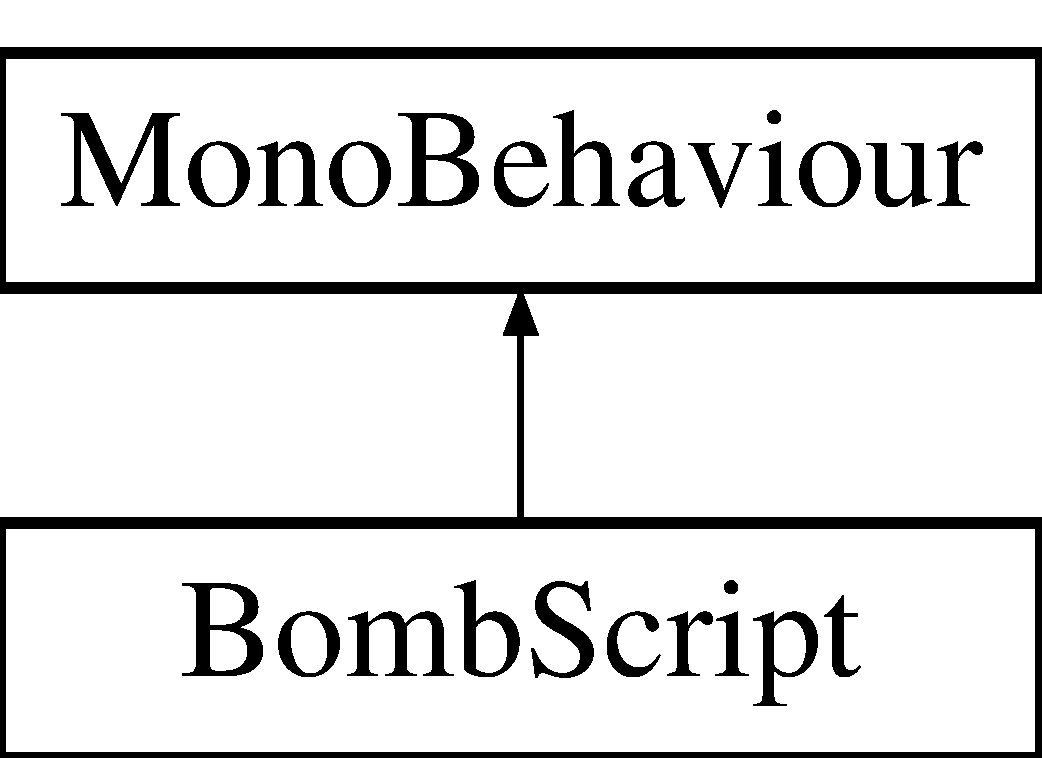
\includegraphics[height=2.000000cm]{classBombScript}
\end{center}
\end{figure}
\subsection*{Public Member Functions}
\begin{DoxyCompactItemize}
\item 
void \hyperlink{classBombScript_af805ef6d3e038e1e677bddd4013d790e}{Start} ()
\begin{DoxyCompactList}\small\item\em Stuff to do at the start, gets attached animator and audio source \end{DoxyCompactList}\item 
void \hyperlink{classBombScript_ac503477a92904905bd3940a5f88dae7b}{Update} ()
\begin{DoxyCompactList}\small\item\em Updates per frame, moves object left per frame, checks if dead, if true, starts death animation\& sound then destroys object \end{DoxyCompactList}\item 
void \hyperlink{classBombScript_ad2919ec2099dd9b523c9f19e8331cb89}{On\-Trigger\-Enter} (Collider col)
\end{DoxyCompactItemize}
\subsection*{Public Attributes}
\begin{DoxyCompactItemize}
\item 
Animator \hyperlink{classBombScript_ad035f9b68c323985dfe3e6a77b01f252}{Bomb\-Enemy}
\begin{DoxyCompactList}\small\item\em The bomb enemy. \end{DoxyCompactList}\item 
Audio\-Source \hyperlink{classBombScript_a1c1f970bb78dc842d25b57d37c963c0e}{Explosion\-S\-D}
\begin{DoxyCompactList}\small\item\em The explosion S. \end{DoxyCompactList}\item 
float \hyperlink{classBombScript_afba19f8bfc4dcd938590b616b81de052}{Enemy\-Speed} = 0.\-1f
\begin{DoxyCompactList}\small\item\em The enemy speed. \end{DoxyCompactList}\end{DoxyCompactItemize}


\subsection{Member Function Documentation}
\hypertarget{classBombScript_ad2919ec2099dd9b523c9f19e8331cb89}{\index{Bomb\-Script@{Bomb\-Script}!On\-Trigger\-Enter@{On\-Trigger\-Enter}}
\index{On\-Trigger\-Enter@{On\-Trigger\-Enter}!BombScript@{Bomb\-Script}}
\subsubsection[{On\-Trigger\-Enter}]{\setlength{\rightskip}{0pt plus 5cm}void Bomb\-Script.\-On\-Trigger\-Enter (
\begin{DoxyParamCaption}
\item[{Collider}]{col}
\end{DoxyParamCaption}
)\hspace{0.3cm}{\ttfamily [inline]}}}\label{classBombScript_ad2919ec2099dd9b523c9f19e8331cb89}




Raises the trigger enter event. 


\begin{DoxyParams}{Parameters}
{\em col} & Col collision parameter to detect collisions\\
\hline
{\em return} & Tag \char`\"{}\-Player\char`\"{} collision causes \hyperlink{classHealth}{Health} call, Dmg received \& object destruct\\
\hline
\end{DoxyParams}
\hypertarget{classBombScript_af805ef6d3e038e1e677bddd4013d790e}{\index{Bomb\-Script@{Bomb\-Script}!Start@{Start}}
\index{Start@{Start}!BombScript@{Bomb\-Script}}
\subsubsection[{Start}]{\setlength{\rightskip}{0pt plus 5cm}void Bomb\-Script.\-Start (
\begin{DoxyParamCaption}
{}
\end{DoxyParamCaption}
)\hspace{0.3cm}{\ttfamily [inline]}}}\label{classBombScript_af805ef6d3e038e1e677bddd4013d790e}


Stuff to do at the start, gets attached animator and audio source 

\hypertarget{classBombScript_ac503477a92904905bd3940a5f88dae7b}{\index{Bomb\-Script@{Bomb\-Script}!Update@{Update}}
\index{Update@{Update}!BombScript@{Bomb\-Script}}
\subsubsection[{Update}]{\setlength{\rightskip}{0pt plus 5cm}void Bomb\-Script.\-Update (
\begin{DoxyParamCaption}
{}
\end{DoxyParamCaption}
)\hspace{0.3cm}{\ttfamily [inline]}}}\label{classBombScript_ac503477a92904905bd3940a5f88dae7b}


Updates per frame, moves object left per frame, checks if dead, if true, starts death animation\& sound then destroys object 



\subsection{Member Data Documentation}
\hypertarget{classBombScript_ad035f9b68c323985dfe3e6a77b01f252}{\index{Bomb\-Script@{Bomb\-Script}!Bomb\-Enemy@{Bomb\-Enemy}}
\index{Bomb\-Enemy@{Bomb\-Enemy}!BombScript@{Bomb\-Script}}
\subsubsection[{Bomb\-Enemy}]{\setlength{\rightskip}{0pt plus 5cm}Animator Bomb\-Script.\-Bomb\-Enemy}}\label{classBombScript_ad035f9b68c323985dfe3e6a77b01f252}


The bomb enemy. 

\hypertarget{classBombScript_afba19f8bfc4dcd938590b616b81de052}{\index{Bomb\-Script@{Bomb\-Script}!Enemy\-Speed@{Enemy\-Speed}}
\index{Enemy\-Speed@{Enemy\-Speed}!BombScript@{Bomb\-Script}}
\subsubsection[{Enemy\-Speed}]{\setlength{\rightskip}{0pt plus 5cm}float Bomb\-Script.\-Enemy\-Speed = 0.\-1f}}\label{classBombScript_afba19f8bfc4dcd938590b616b81de052}


The enemy speed. 

\hypertarget{classBombScript_a1c1f970bb78dc842d25b57d37c963c0e}{\index{Bomb\-Script@{Bomb\-Script}!Explosion\-S\-D@{Explosion\-S\-D}}
\index{Explosion\-S\-D@{Explosion\-S\-D}!BombScript@{Bomb\-Script}}
\subsubsection[{Explosion\-S\-D}]{\setlength{\rightskip}{0pt plus 5cm}Audio\-Source Bomb\-Script.\-Explosion\-S\-D}}\label{classBombScript_a1c1f970bb78dc842d25b57d37c963c0e}


The explosion S. 



The documentation for this class was generated from the following file\-:\begin{DoxyCompactItemize}
\item 
Bomb\-Script.\-cs\end{DoxyCompactItemize}

\hypertarget{classBullets}{\section{Bullets Class Reference}
\label{classBullets}\index{Bullets@{Bullets}}
}
Inheritance diagram for Bullets\-:\begin{figure}[H]
\begin{center}
\leavevmode
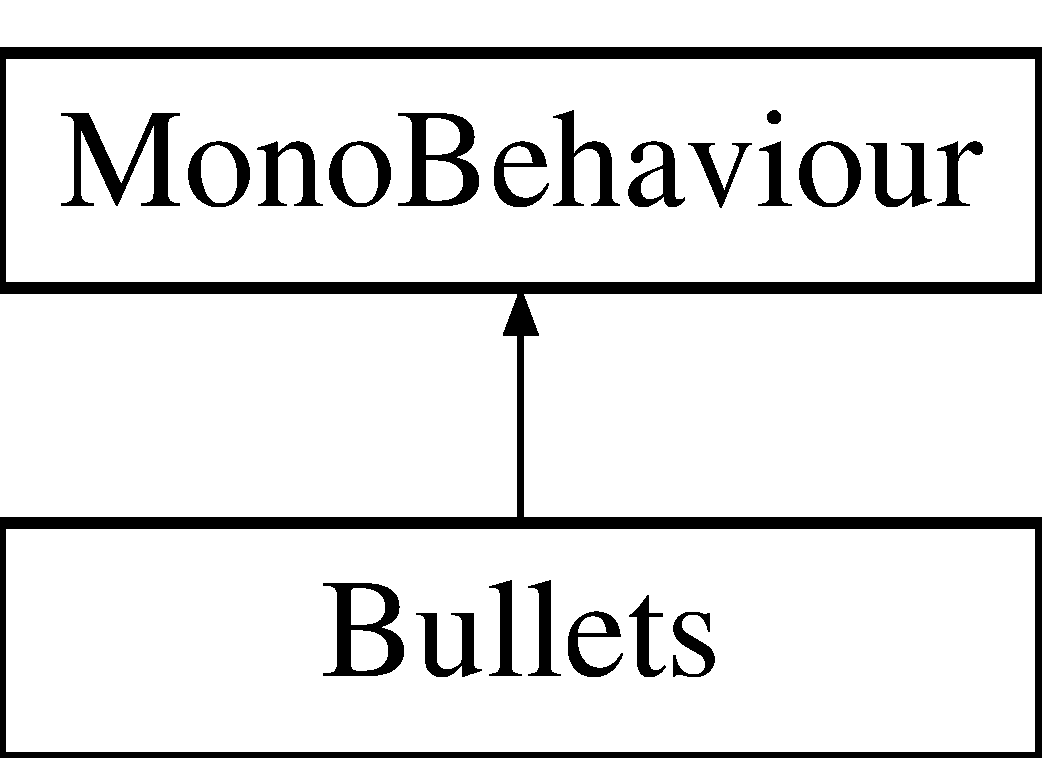
\includegraphics[height=2.000000cm]{classBullets}
\end{center}
\end{figure}
\subsection*{Public Member Functions}
\begin{DoxyCompactItemize}
\item 
void \hyperlink{classBullets_a5f8f1e6e26692c4309d245bfc82f262d}{Update} ()
\begin{DoxyCompactList}\small\item\em Update called once per frame, moves object right, destroys object after certain time \end{DoxyCompactList}\item 
void \hyperlink{classBullets_a15349b695ed15b96eda82606d5da773e}{On\-Trigger\-Enter} (Collider Hit)
\begin{DoxyCompactList}\small\item\em Collider trigger, on hit do something \end{DoxyCompactList}\end{DoxyCompactItemize}
\subsection*{Public Attributes}
\begin{DoxyCompactItemize}
\item 
float \hyperlink{classBullets_a9120f537885ce71eb6bda1fdc4c4bdba}{Bulletspeed} = 5
\begin{DoxyCompactList}\small\item\em The bulletspeed. \end{DoxyCompactList}\item 
float \hyperlink{classBullets_acc3d972e4c08788a0aff8b87faf7c3a6}{Dmg} = 5
\begin{DoxyCompactList}\small\item\em The damage. \end{DoxyCompactList}\end{DoxyCompactItemize}


\subsection{Member Function Documentation}
\hypertarget{classBullets_a15349b695ed15b96eda82606d5da773e}{\index{Bullets@{Bullets}!On\-Trigger\-Enter@{On\-Trigger\-Enter}}
\index{On\-Trigger\-Enter@{On\-Trigger\-Enter}!Bullets@{Bullets}}
\subsubsection[{On\-Trigger\-Enter}]{\setlength{\rightskip}{0pt plus 5cm}void Bullets.\-On\-Trigger\-Enter (
\begin{DoxyParamCaption}
\item[{Collider}]{Hit}
\end{DoxyParamCaption}
)\hspace{0.3cm}{\ttfamily [inline]}}}\label{classBullets_a15349b695ed15b96eda82606d5da773e}


Collider trigger, on hit do something 


\begin{DoxyParams}{Parameters}
{\em Hit} & Hit collision detect\\
\hline
{\em Return} & $>$ If hit is obstacle, destroy object and this, if hit is enemy, enemy is damaged\\
\hline
\end{DoxyParams}
\hypertarget{classBullets_a5f8f1e6e26692c4309d245bfc82f262d}{\index{Bullets@{Bullets}!Update@{Update}}
\index{Update@{Update}!Bullets@{Bullets}}
\subsubsection[{Update}]{\setlength{\rightskip}{0pt plus 5cm}void Bullets.\-Update (
\begin{DoxyParamCaption}
{}
\end{DoxyParamCaption}
)\hspace{0.3cm}{\ttfamily [inline]}}}\label{classBullets_a5f8f1e6e26692c4309d245bfc82f262d}


Update called once per frame, moves object right, destroys object after certain time 



\subsection{Member Data Documentation}
\hypertarget{classBullets_a9120f537885ce71eb6bda1fdc4c4bdba}{\index{Bullets@{Bullets}!Bulletspeed@{Bulletspeed}}
\index{Bulletspeed@{Bulletspeed}!Bullets@{Bullets}}
\subsubsection[{Bulletspeed}]{\setlength{\rightskip}{0pt plus 5cm}float Bullets.\-Bulletspeed = 5}}\label{classBullets_a9120f537885ce71eb6bda1fdc4c4bdba}


The bulletspeed. 

\hypertarget{classBullets_acc3d972e4c08788a0aff8b87faf7c3a6}{\index{Bullets@{Bullets}!Dmg@{Dmg}}
\index{Dmg@{Dmg}!Bullets@{Bullets}}
\subsubsection[{Dmg}]{\setlength{\rightskip}{0pt plus 5cm}float Bullets.\-Dmg = 5}}\label{classBullets_acc3d972e4c08788a0aff8b87faf7c3a6}


The damage. 



The documentation for this class was generated from the following file\-:\begin{DoxyCompactItemize}
\item 
Bullets.\-cs\end{DoxyCompactItemize}

\hypertarget{classDestroyByTime}{\section{Destroy\-By\-Time Class Reference}
\label{classDestroyByTime}\index{Destroy\-By\-Time@{Destroy\-By\-Time}}
}
Inheritance diagram for Destroy\-By\-Time\-:\begin{figure}[H]
\begin{center}
\leavevmode
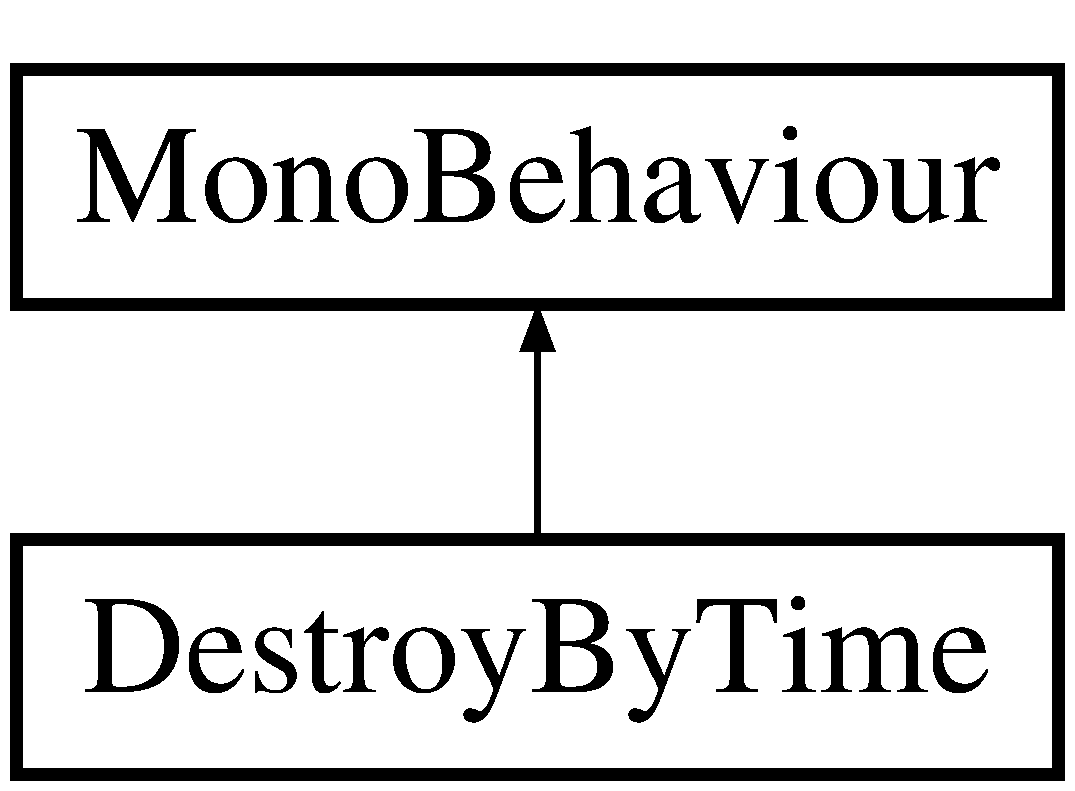
\includegraphics[height=2.000000cm]{classDestroyByTime}
\end{center}
\end{figure}
\subsection*{Public Member Functions}
\begin{DoxyCompactItemize}
\item 
void \hyperlink{classDestroyByTime_a0ac6f52b53d41ea5e4c6ea7a8a832dc9}{Start} ()
\begin{DoxyCompactList}\small\item\em Inititation, destroy object at lifetime \end{DoxyCompactList}\end{DoxyCompactItemize}
\subsection*{Public Attributes}
\begin{DoxyCompactItemize}
\item 
float \hyperlink{classDestroyByTime_a1c11e0a64a46ee1b3eb9e71c1bc5f8c8}{lifetime}
\begin{DoxyCompactList}\small\item\em The lifetime of an object before being destroyed \end{DoxyCompactList}\end{DoxyCompactItemize}


\subsection{Member Function Documentation}
\hypertarget{classDestroyByTime_a0ac6f52b53d41ea5e4c6ea7a8a832dc9}{\index{Destroy\-By\-Time@{Destroy\-By\-Time}!Start@{Start}}
\index{Start@{Start}!DestroyByTime@{Destroy\-By\-Time}}
\subsubsection[{Start}]{\setlength{\rightskip}{0pt plus 5cm}void Destroy\-By\-Time.\-Start (
\begin{DoxyParamCaption}
{}
\end{DoxyParamCaption}
)\hspace{0.3cm}{\ttfamily [inline]}}}\label{classDestroyByTime_a0ac6f52b53d41ea5e4c6ea7a8a832dc9}


Inititation, destroy object at lifetime 



\subsection{Member Data Documentation}
\hypertarget{classDestroyByTime_a1c11e0a64a46ee1b3eb9e71c1bc5f8c8}{\index{Destroy\-By\-Time@{Destroy\-By\-Time}!lifetime@{lifetime}}
\index{lifetime@{lifetime}!DestroyByTime@{Destroy\-By\-Time}}
\subsubsection[{lifetime}]{\setlength{\rightskip}{0pt plus 5cm}float Destroy\-By\-Time.\-lifetime}}\label{classDestroyByTime_a1c11e0a64a46ee1b3eb9e71c1bc5f8c8}


The lifetime of an object before being destroyed 



The documentation for this class was generated from the following file\-:\begin{DoxyCompactItemize}
\item 
Destroy\-By\-Time.\-cs\end{DoxyCompactItemize}

\hypertarget{classGameCamera}{\section{Game\-Camera Class Reference}
\label{classGameCamera}\index{Game\-Camera@{Game\-Camera}}
}
Inheritance diagram for Game\-Camera\-:\begin{figure}[H]
\begin{center}
\leavevmode
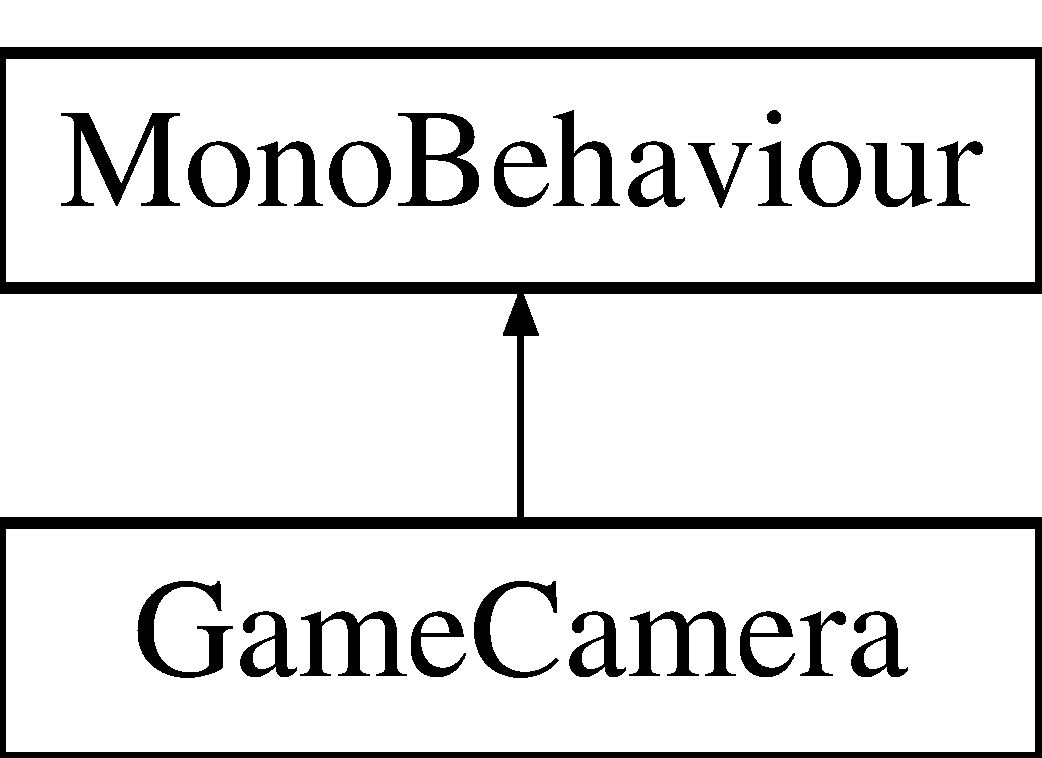
\includegraphics[height=2.000000cm]{classGameCamera}
\end{center}
\end{figure}
\subsection*{Public Member Functions}
\begin{DoxyCompactItemize}
\item 
void \hyperlink{classGameCamera_adb2bfc4c2738e33d9b98bc97fddacb4e}{Set\-Target} (Transform t)
\begin{DoxyCompactList}\small\item\em Sets the target to aim for \end{DoxyCompactList}\item 
void \hyperlink{classGameCamera_aa6ef15e6deb0f8921cdb93c9ad719ca0}{Update} ()
\begin{DoxyCompactList}\small\item\em Update per frame, transforms object to target vector \end{DoxyCompactList}\item 
float \hyperlink{classGameCamera_adb57e107c5ac3c860c1d31589453c9a4}{Increment\-Towards} (float n, float \hyperlink{classGameCamera_a952c82b1dd2710a4af6fe0fbeaca776c}{target}, float a)
\begin{DoxyCompactList}\small\item\em Increments param n towards target by speed \end{DoxyCompactList}\end{DoxyCompactItemize}
\subsection*{Public Attributes}
\begin{DoxyCompactItemize}
\item 
Transform \hyperlink{classGameCamera_a952c82b1dd2710a4af6fe0fbeaca776c}{target}
\begin{DoxyCompactList}\small\item\em vector target to aim for \end{DoxyCompactList}\item 
float \hyperlink{classGameCamera_af9039782e227fc39fa15528908e37137}{track\-Speed} = 10
\begin{DoxyCompactList}\small\item\em The track speed. \end{DoxyCompactList}\end{DoxyCompactItemize}


\subsection{Member Function Documentation}
\hypertarget{classGameCamera_adb57e107c5ac3c860c1d31589453c9a4}{\index{Game\-Camera@{Game\-Camera}!Increment\-Towards@{Increment\-Towards}}
\index{Increment\-Towards@{Increment\-Towards}!GameCamera@{Game\-Camera}}
\subsubsection[{Increment\-Towards}]{\setlength{\rightskip}{0pt plus 5cm}float Game\-Camera.\-Increment\-Towards (
\begin{DoxyParamCaption}
\item[{float}]{n, }
\item[{float}]{target, }
\item[{float}]{a}
\end{DoxyParamCaption}
)\hspace{0.3cm}{\ttfamily [inline]}}}\label{classGameCamera_adb57e107c5ac3c860c1d31589453c9a4}


Increments param n towards target by speed 

\begin{DoxyReturn}{Returns}
The towards.
\end{DoxyReturn}

\begin{DoxyParams}{Parameters}
{\em n} & First vector, current position vector of cam\\
\hline
{\em target} & Second vector, target vector for cam\\
\hline
{\em a} & The alpha component.\\
\hline
\end{DoxyParams}
\hypertarget{classGameCamera_adb2bfc4c2738e33d9b98bc97fddacb4e}{\index{Game\-Camera@{Game\-Camera}!Set\-Target@{Set\-Target}}
\index{Set\-Target@{Set\-Target}!GameCamera@{Game\-Camera}}
\subsubsection[{Set\-Target}]{\setlength{\rightskip}{0pt plus 5cm}void Game\-Camera.\-Set\-Target (
\begin{DoxyParamCaption}
\item[{Transform}]{t}
\end{DoxyParamCaption}
)\hspace{0.3cm}{\ttfamily [inline]}}}\label{classGameCamera_adb2bfc4c2738e33d9b98bc97fddacb4e}


Sets the target to aim for 


\begin{DoxyParams}{Parameters}
{\em t} & vector to aim for\\
\hline
\end{DoxyParams}
\hypertarget{classGameCamera_aa6ef15e6deb0f8921cdb93c9ad719ca0}{\index{Game\-Camera@{Game\-Camera}!Update@{Update}}
\index{Update@{Update}!GameCamera@{Game\-Camera}}
\subsubsection[{Update}]{\setlength{\rightskip}{0pt plus 5cm}void Game\-Camera.\-Update (
\begin{DoxyParamCaption}
{}
\end{DoxyParamCaption}
)\hspace{0.3cm}{\ttfamily [inline]}}}\label{classGameCamera_aa6ef15e6deb0f8921cdb93c9ad719ca0}


Update per frame, transforms object to target vector 



\subsection{Member Data Documentation}
\hypertarget{classGameCamera_a952c82b1dd2710a4af6fe0fbeaca776c}{\index{Game\-Camera@{Game\-Camera}!target@{target}}
\index{target@{target}!GameCamera@{Game\-Camera}}
\subsubsection[{target}]{\setlength{\rightskip}{0pt plus 5cm}Transform Game\-Camera.\-target}}\label{classGameCamera_a952c82b1dd2710a4af6fe0fbeaca776c}


vector target to aim for 

\hypertarget{classGameCamera_af9039782e227fc39fa15528908e37137}{\index{Game\-Camera@{Game\-Camera}!track\-Speed@{track\-Speed}}
\index{track\-Speed@{track\-Speed}!GameCamera@{Game\-Camera}}
\subsubsection[{track\-Speed}]{\setlength{\rightskip}{0pt plus 5cm}float Game\-Camera.\-track\-Speed = 10}}\label{classGameCamera_af9039782e227fc39fa15528908e37137}


The track speed. 



The documentation for this class was generated from the following file\-:\begin{DoxyCompactItemize}
\item 
Game\-Camera.\-cs\end{DoxyCompactItemize}

\hypertarget{classGameController}{\section{Game\-Controller Class Reference}
\label{classGameController}\index{Game\-Controller@{Game\-Controller}}
}
Inheritance diagram for Game\-Controller\-:\begin{figure}[H]
\begin{center}
\leavevmode
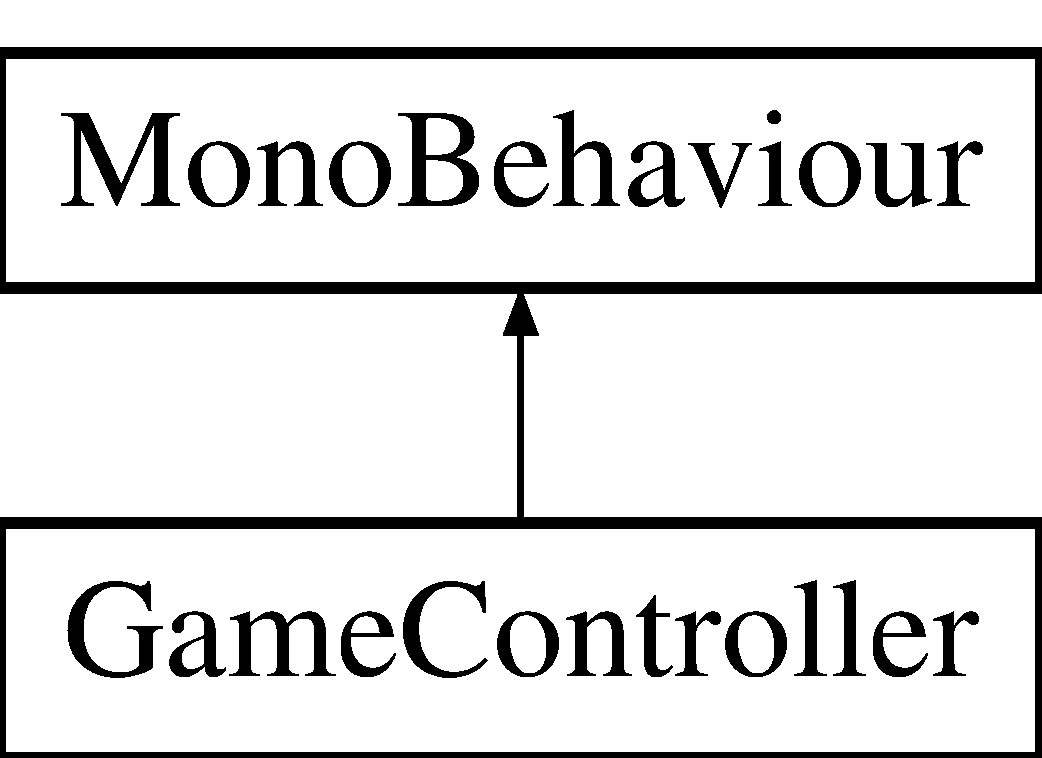
\includegraphics[height=2.000000cm]{classGameController}
\end{center}
\end{figure}
\subsection*{Public Member Functions}
\begin{DoxyCompactItemize}
\item 
void \hyperlink{classGameController_a5a89277529cadb49af7d55eba3bbf056}{Update} ()
\begin{DoxyCompactList}\small\item\em Update per frame, randomizer for spawning between objects \end{DoxyCompactList}\item 
void \hyperlink{classGameController_a97788a7aa0f09c8d748781683e5f045b}{Start} ()
\begin{DoxyCompactList}\small\item\em initializer to start time for waves, sets hazards to spawn, spawn time, wave time and position to spawn \end{DoxyCompactList}\end{DoxyCompactItemize}
\subsection*{Public Attributes}
\begin{DoxyCompactItemize}
\item 
Game\-Object \hyperlink{classGameController_ae2d31db5ff00946e41b2dcd7ddda941a}{Object1}
\begin{DoxyCompactList}\small\item\em 1st Placement for game\-Object spawning. \end{DoxyCompactList}\item 
Game\-Object \hyperlink{classGameController_ab5c9311e9997c3d8a34833b3760f28f8}{Object2}
\begin{DoxyCompactList}\small\item\em 2nd Placement for game\-Object spawning. \end{DoxyCompactList}\item 
Game\-Object \hyperlink{classGameController_a9956f5a361f097e051a144a2b787e5ca}{Object3}
\begin{DoxyCompactList}\small\item\em 3rd Placement for game\-Object spawning. \end{DoxyCompactList}\item 
Game\-Object \hyperlink{classGameController_a77c185a594a084fe342e8de517808654}{hazard}
\begin{DoxyCompactList}\small\item\em Hazard spot for randomizing between 3 objects. \end{DoxyCompactList}\item 
Vector3 \hyperlink{classGameController_a5e4f56c23896d4b528da579f93335896}{spawn\-Values}
\begin{DoxyCompactList}\small\item\em The spawn values. \end{DoxyCompactList}\item 
int \hyperlink{classGameController_a973f0e7d25e3b260cf0aa51730584ada}{hazard\-Count}
\begin{DoxyCompactList}\small\item\em The hazard count. \end{DoxyCompactList}\item 
float \hyperlink{classGameController_a27c91a14de3982813ad3d8245d0134d7}{spawn\-Wait}
\begin{DoxyCompactList}\small\item\em The spawn wait. \end{DoxyCompactList}\item 
float \hyperlink{classGameController_a9b6f96c29d3ee0f2c692c30ed2b12835}{start\-Wait}
\begin{DoxyCompactList}\small\item\em The start wait. \end{DoxyCompactList}\item 
float \hyperlink{classGameController_ad210270b367c1c439d35e8177d989019}{wave\-Wait}
\begin{DoxyCompactList}\small\item\em The wave wait. \end{DoxyCompactList}\item 
\hypertarget{classGameController_a874a60a231abb44f54f0b260c93be52b}{int \hyperlink{classGameController_a874a60a231abb44f54f0b260c93be52b}{choice}}\label{classGameController_a874a60a231abb44f54f0b260c93be52b}

\begin{DoxyCompactList}\small\item\em Float Randomizer for objects summary$>$ \end{DoxyCompactList}\end{DoxyCompactItemize}


\subsection{Member Function Documentation}
\hypertarget{classGameController_a97788a7aa0f09c8d748781683e5f045b}{\index{Game\-Controller@{Game\-Controller}!Start@{Start}}
\index{Start@{Start}!GameController@{Game\-Controller}}
\subsubsection[{Start}]{\setlength{\rightskip}{0pt plus 5cm}void Game\-Controller.\-Start (
\begin{DoxyParamCaption}
{}
\end{DoxyParamCaption}
)\hspace{0.3cm}{\ttfamily [inline]}}}\label{classGameController_a97788a7aa0f09c8d748781683e5f045b}


initializer to start time for waves, sets hazards to spawn, spawn time, wave time and position to spawn 

\hypertarget{classGameController_a5a89277529cadb49af7d55eba3bbf056}{\index{Game\-Controller@{Game\-Controller}!Update@{Update}}
\index{Update@{Update}!GameController@{Game\-Controller}}
\subsubsection[{Update}]{\setlength{\rightskip}{0pt plus 5cm}void Game\-Controller.\-Update (
\begin{DoxyParamCaption}
{}
\end{DoxyParamCaption}
)\hspace{0.3cm}{\ttfamily [inline]}}}\label{classGameController_a5a89277529cadb49af7d55eba3bbf056}


Update per frame, randomizer for spawning between objects 



\subsection{Member Data Documentation}
\hypertarget{classGameController_a77c185a594a084fe342e8de517808654}{\index{Game\-Controller@{Game\-Controller}!hazard@{hazard}}
\index{hazard@{hazard}!GameController@{Game\-Controller}}
\subsubsection[{hazard}]{\setlength{\rightskip}{0pt plus 5cm}Game\-Object Game\-Controller.\-hazard}}\label{classGameController_a77c185a594a084fe342e8de517808654}


Hazard spot for randomizing between 3 objects. 

\hypertarget{classGameController_a973f0e7d25e3b260cf0aa51730584ada}{\index{Game\-Controller@{Game\-Controller}!hazard\-Count@{hazard\-Count}}
\index{hazard\-Count@{hazard\-Count}!GameController@{Game\-Controller}}
\subsubsection[{hazard\-Count}]{\setlength{\rightskip}{0pt plus 5cm}int Game\-Controller.\-hazard\-Count}}\label{classGameController_a973f0e7d25e3b260cf0aa51730584ada}


The hazard count. 

\hypertarget{classGameController_ae2d31db5ff00946e41b2dcd7ddda941a}{\index{Game\-Controller@{Game\-Controller}!Object1@{Object1}}
\index{Object1@{Object1}!GameController@{Game\-Controller}}
\subsubsection[{Object1}]{\setlength{\rightskip}{0pt plus 5cm}Game\-Object Game\-Controller.\-Object1}}\label{classGameController_ae2d31db5ff00946e41b2dcd7ddda941a}


1st Placement for game\-Object spawning. 

\hypertarget{classGameController_ab5c9311e9997c3d8a34833b3760f28f8}{\index{Game\-Controller@{Game\-Controller}!Object2@{Object2}}
\index{Object2@{Object2}!GameController@{Game\-Controller}}
\subsubsection[{Object2}]{\setlength{\rightskip}{0pt plus 5cm}Game\-Object Game\-Controller.\-Object2}}\label{classGameController_ab5c9311e9997c3d8a34833b3760f28f8}


2nd Placement for game\-Object spawning. 

\hypertarget{classGameController_a9956f5a361f097e051a144a2b787e5ca}{\index{Game\-Controller@{Game\-Controller}!Object3@{Object3}}
\index{Object3@{Object3}!GameController@{Game\-Controller}}
\subsubsection[{Object3}]{\setlength{\rightskip}{0pt plus 5cm}Game\-Object Game\-Controller.\-Object3}}\label{classGameController_a9956f5a361f097e051a144a2b787e5ca}


3rd Placement for game\-Object spawning. 

\hypertarget{classGameController_a5e4f56c23896d4b528da579f93335896}{\index{Game\-Controller@{Game\-Controller}!spawn\-Values@{spawn\-Values}}
\index{spawn\-Values@{spawn\-Values}!GameController@{Game\-Controller}}
\subsubsection[{spawn\-Values}]{\setlength{\rightskip}{0pt plus 5cm}Vector3 Game\-Controller.\-spawn\-Values}}\label{classGameController_a5e4f56c23896d4b528da579f93335896}


The spawn values. 

\hypertarget{classGameController_a27c91a14de3982813ad3d8245d0134d7}{\index{Game\-Controller@{Game\-Controller}!spawn\-Wait@{spawn\-Wait}}
\index{spawn\-Wait@{spawn\-Wait}!GameController@{Game\-Controller}}
\subsubsection[{spawn\-Wait}]{\setlength{\rightskip}{0pt plus 5cm}float Game\-Controller.\-spawn\-Wait}}\label{classGameController_a27c91a14de3982813ad3d8245d0134d7}


The spawn wait. 

\hypertarget{classGameController_a9b6f96c29d3ee0f2c692c30ed2b12835}{\index{Game\-Controller@{Game\-Controller}!start\-Wait@{start\-Wait}}
\index{start\-Wait@{start\-Wait}!GameController@{Game\-Controller}}
\subsubsection[{start\-Wait}]{\setlength{\rightskip}{0pt plus 5cm}float Game\-Controller.\-start\-Wait}}\label{classGameController_a9b6f96c29d3ee0f2c692c30ed2b12835}


The start wait. 

\hypertarget{classGameController_ad210270b367c1c439d35e8177d989019}{\index{Game\-Controller@{Game\-Controller}!wave\-Wait@{wave\-Wait}}
\index{wave\-Wait@{wave\-Wait}!GameController@{Game\-Controller}}
\subsubsection[{wave\-Wait}]{\setlength{\rightskip}{0pt plus 5cm}float Game\-Controller.\-wave\-Wait}}\label{classGameController_ad210270b367c1c439d35e8177d989019}


The wave wait. 



The documentation for this class was generated from the following file\-:\begin{DoxyCompactItemize}
\item 
Game\-Controller.\-cs\end{DoxyCompactItemize}

\hypertarget{classGameManager}{\section{Game\-Manager Class Reference}
\label{classGameManager}\index{Game\-Manager@{Game\-Manager}}
}
Inheritance diagram for Game\-Manager\-:\begin{figure}[H]
\begin{center}
\leavevmode
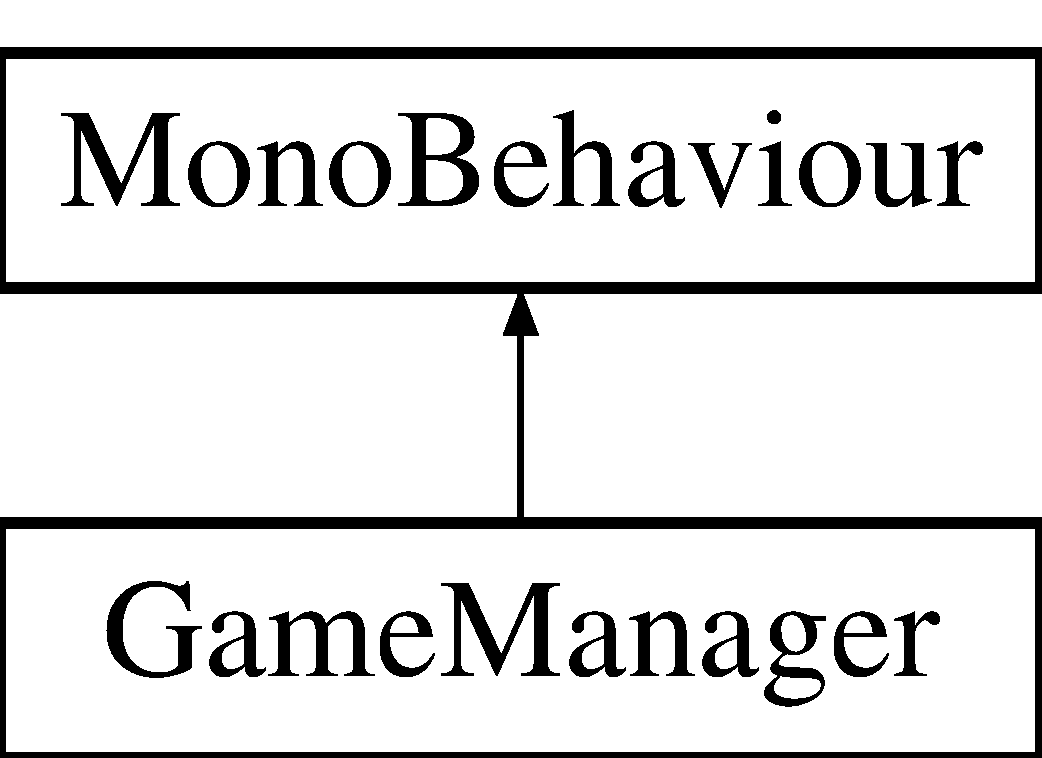
\includegraphics[height=2.000000cm]{classGameManager}
\end{center}
\end{figure}
\subsection*{Public Member Functions}
\begin{DoxyCompactItemize}
\item 
void \hyperlink{classGameManager_a5ccfacd027ad08eeb4ff1f25a7f59c98}{Start} ()
\begin{DoxyCompactList}\small\item\em At start, get attached gameobject and spawn player \end{DoxyCompactList}\item 
void \hyperlink{classGameManager_a62960104332e06a3324eb2cc78ce4317}{Spawn\-Player} ()
\begin{DoxyCompactList}\small\item\em Spawns the player and sets camera on player \end{DoxyCompactList}\end{DoxyCompactItemize}
\subsection*{Public Attributes}
\begin{DoxyCompactItemize}
\item 
Game\-Object \hyperlink{classGameManager_abe8e79771775bc67c63c4ac43349dc8a}{player}
\begin{DoxyCompactList}\small\item\em Gameobject spot to place player. \end{DoxyCompactList}\item 
\hyperlink{classGameCamera}{Game\-Camera} \hyperlink{classGameManager_ad95999a7d419e9262f7f22fdad69df9d}{cam}
\begin{DoxyCompactList}\small\item\em Gameobject camera. \end{DoxyCompactList}\end{DoxyCompactItemize}


\subsection{Member Function Documentation}
\hypertarget{classGameManager_a62960104332e06a3324eb2cc78ce4317}{\index{Game\-Manager@{Game\-Manager}!Spawn\-Player@{Spawn\-Player}}
\index{Spawn\-Player@{Spawn\-Player}!GameManager@{Game\-Manager}}
\subsubsection[{Spawn\-Player}]{\setlength{\rightskip}{0pt plus 5cm}void Game\-Manager.\-Spawn\-Player (
\begin{DoxyParamCaption}
{}
\end{DoxyParamCaption}
)\hspace{0.3cm}{\ttfamily [inline]}}}\label{classGameManager_a62960104332e06a3324eb2cc78ce4317}


Spawns the player and sets camera on player 

\hypertarget{classGameManager_a5ccfacd027ad08eeb4ff1f25a7f59c98}{\index{Game\-Manager@{Game\-Manager}!Start@{Start}}
\index{Start@{Start}!GameManager@{Game\-Manager}}
\subsubsection[{Start}]{\setlength{\rightskip}{0pt plus 5cm}void Game\-Manager.\-Start (
\begin{DoxyParamCaption}
{}
\end{DoxyParamCaption}
)\hspace{0.3cm}{\ttfamily [inline]}}}\label{classGameManager_a5ccfacd027ad08eeb4ff1f25a7f59c98}


At start, get attached gameobject and spawn player 



\subsection{Member Data Documentation}
\hypertarget{classGameManager_ad95999a7d419e9262f7f22fdad69df9d}{\index{Game\-Manager@{Game\-Manager}!cam@{cam}}
\index{cam@{cam}!GameManager@{Game\-Manager}}
\subsubsection[{cam}]{\setlength{\rightskip}{0pt plus 5cm}{\bf Game\-Camera} Game\-Manager.\-cam}}\label{classGameManager_ad95999a7d419e9262f7f22fdad69df9d}


Gameobject camera. 

\hypertarget{classGameManager_abe8e79771775bc67c63c4ac43349dc8a}{\index{Game\-Manager@{Game\-Manager}!player@{player}}
\index{player@{player}!GameManager@{Game\-Manager}}
\subsubsection[{player}]{\setlength{\rightskip}{0pt plus 5cm}Game\-Object Game\-Manager.\-player}}\label{classGameManager_abe8e79771775bc67c63c4ac43349dc8a}


Gameobject spot to place player. 



The documentation for this class was generated from the following file\-:\begin{DoxyCompactItemize}
\item 
Game\-Manager.\-cs\end{DoxyCompactItemize}

\hypertarget{classHealth}{\section{Health Class Reference}
\label{classHealth}\index{Health@{Health}}
}
Inheritance diagram for Health\-:\begin{figure}[H]
\begin{center}
\leavevmode
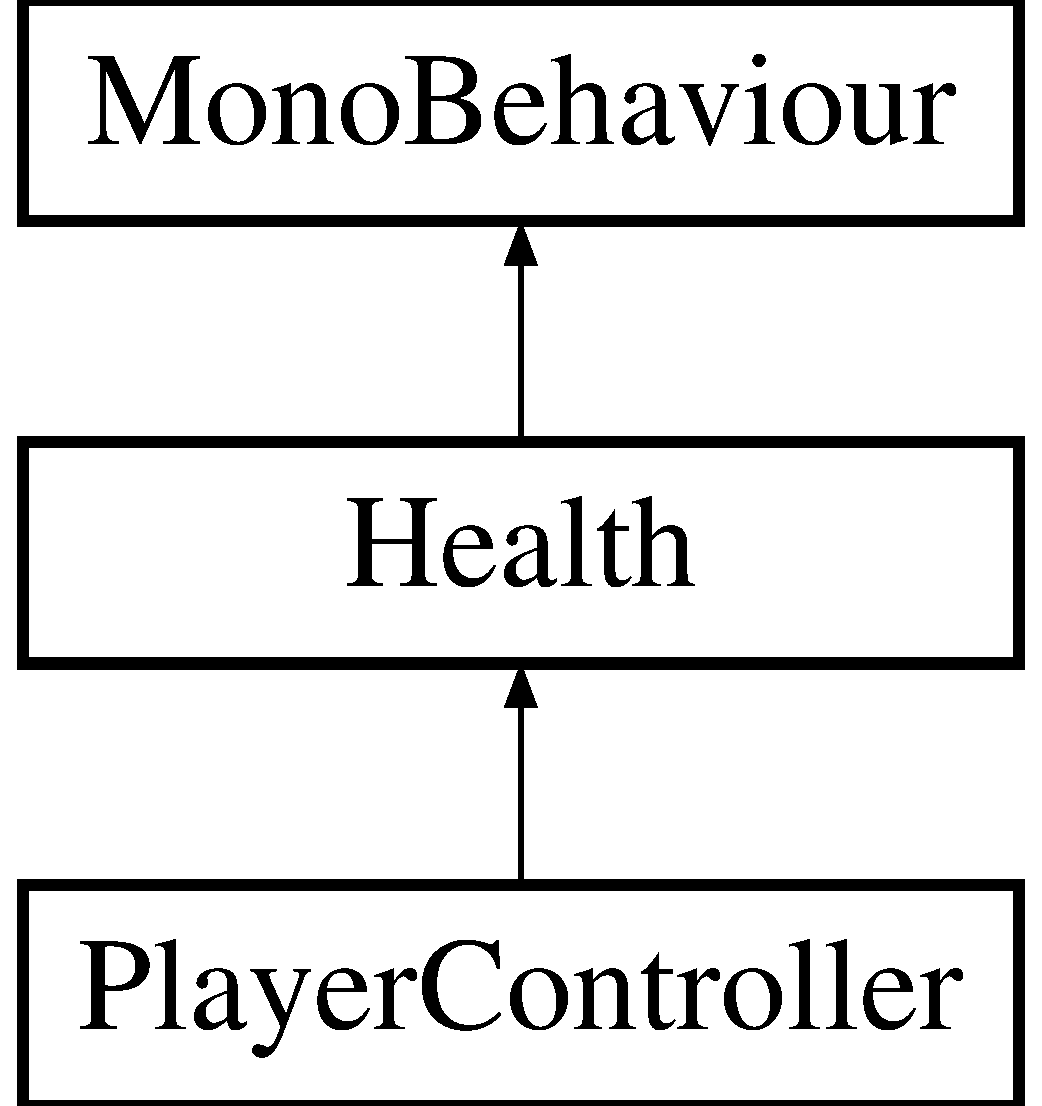
\includegraphics[height=3.000000cm]{classHealth}
\end{center}
\end{figure}
\subsection*{Public Member Functions}
\begin{DoxyCompactItemize}
\item 
void \hyperlink{classHealth_a0c741273cc605c39ec6fbe1f7afc208f}{Receive\-Dmg} (float dmg)
\begin{DoxyCompactList}\small\item\em Damage function, subtracts dmg from current health /// \end{DoxyCompactList}\item 
bool \hyperlink{classHealth_a3bb9917bfd54064704c2a282505a5dbb}{is\-Dead} ()
\begin{DoxyCompactList}\small\item\em Checks if the object is dead depending on current health /// \end{DoxyCompactList}\end{DoxyCompactItemize}
\subsection*{Public Attributes}
\begin{DoxyCompactItemize}
\item 
float \hyperlink{classHealth_a68c8d8201a5d0117cfc647c6a6c0c454}{current\-Health}
\begin{DoxyCompactList}\small\item\em The current health. \end{DoxyCompactList}\end{DoxyCompactItemize}


\subsection{Member Function Documentation}
\hypertarget{classHealth_a3bb9917bfd54064704c2a282505a5dbb}{\index{Health@{Health}!is\-Dead@{is\-Dead}}
\index{is\-Dead@{is\-Dead}!Health@{Health}}
\subsubsection[{is\-Dead}]{\setlength{\rightskip}{0pt plus 5cm}bool Health.\-is\-Dead (
\begin{DoxyParamCaption}
{}
\end{DoxyParamCaption}
)\hspace{0.3cm}{\ttfamily [inline]}}}\label{classHealth_a3bb9917bfd54064704c2a282505a5dbb}


Checks if the object is dead depending on current health /// 

\begin{DoxyReturn}{Returns}
{\ttfamily true}, if dead was dead, {\ttfamily false} target is still alive.
\end{DoxyReturn}
\hypertarget{classHealth_a0c741273cc605c39ec6fbe1f7afc208f}{\index{Health@{Health}!Receive\-Dmg@{Receive\-Dmg}}
\index{Receive\-Dmg@{Receive\-Dmg}!Health@{Health}}
\subsubsection[{Receive\-Dmg}]{\setlength{\rightskip}{0pt plus 5cm}void Health.\-Receive\-Dmg (
\begin{DoxyParamCaption}
\item[{float}]{dmg}
\end{DoxyParamCaption}
)\hspace{0.3cm}{\ttfamily [inline]}}}\label{classHealth_a0c741273cc605c39ec6fbe1f7afc208f}


Damage function, subtracts dmg from current health /// 


\begin{DoxyParams}{Parameters}
{\em dmg} & Damage to take\\
\hline
\end{DoxyParams}


\subsection{Member Data Documentation}
\hypertarget{classHealth_a68c8d8201a5d0117cfc647c6a6c0c454}{\index{Health@{Health}!current\-Health@{current\-Health}}
\index{current\-Health@{current\-Health}!Health@{Health}}
\subsubsection[{current\-Health}]{\setlength{\rightskip}{0pt plus 5cm}float Health.\-current\-Health}}\label{classHealth_a68c8d8201a5d0117cfc647c6a6c0c454}


The current health. 



The documentation for this class was generated from the following file\-:\begin{DoxyCompactItemize}
\item 
Health.\-cs\end{DoxyCompactItemize}

\hypertarget{classMedPack}{\section{Med\-Pack Class Reference}
\label{classMedPack}\index{Med\-Pack@{Med\-Pack}}
}
Inheritance diagram for Med\-Pack\-:\begin{figure}[H]
\begin{center}
\leavevmode
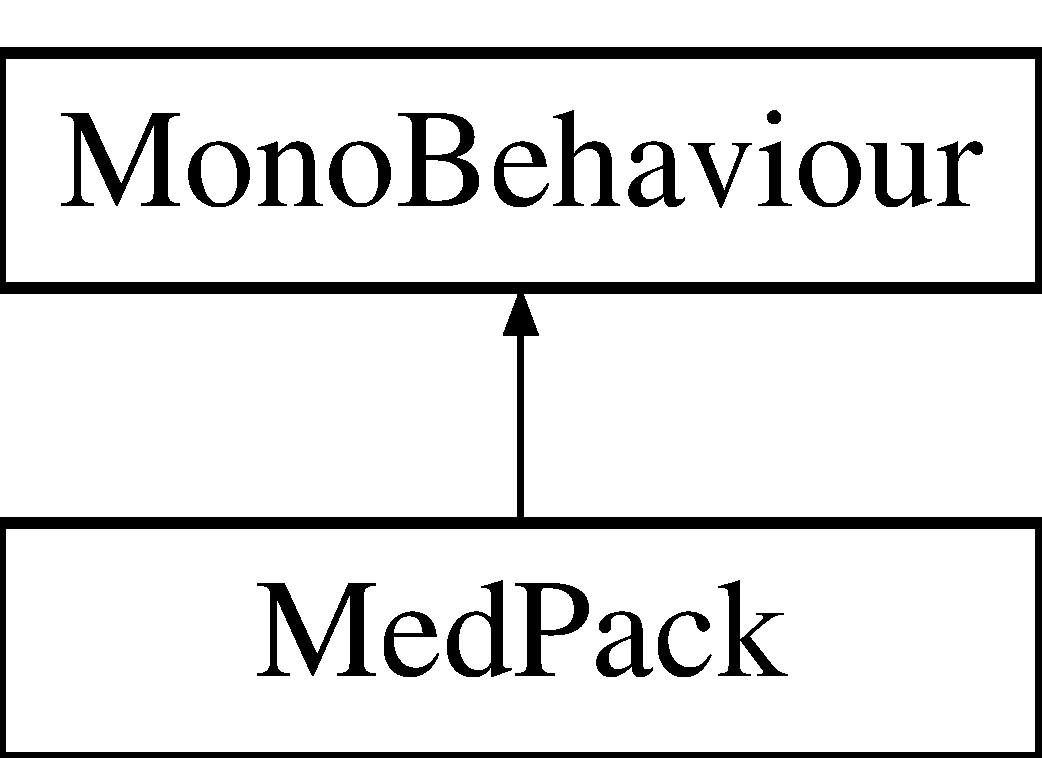
\includegraphics[height=2.000000cm]{classMedPack}
\end{center}
\end{figure}
\subsection*{Public Member Functions}
\begin{DoxyCompactItemize}
\item 
void \hyperlink{classMedPack_ab62bb43788d62cadf3177f763ee14820}{Update} ()
\begin{DoxyCompactList}\small\item\em Updates per frame, moves object left \end{DoxyCompactList}\item 
void \hyperlink{classMedPack_ae69e19d12dce004d6974e23aed815e7f}{On\-Trigger\-Enter} (Collider col)
\begin{DoxyCompactList}\small\item\em Object trigger on collision \end{DoxyCompactList}\end{DoxyCompactItemize}
\subsection*{Public Attributes}
\begin{DoxyCompactItemize}
\item 
float \hyperlink{classMedPack_a054a06495e6562f93eaeefed24d1d474}{Med\-Speed} = 0.\-1f
\begin{DoxyCompactList}\small\item\em The medpack speed. \end{DoxyCompactList}\item 
float \hyperlink{classMedPack_a7d896451dc580637510d0d345db611da}{Heal\-A\-M\-T} = 2
\begin{DoxyCompactList}\small\item\em The total heal amount. \end{DoxyCompactList}\end{DoxyCompactItemize}


\subsection{Member Function Documentation}
\hypertarget{classMedPack_ae69e19d12dce004d6974e23aed815e7f}{\index{Med\-Pack@{Med\-Pack}!On\-Trigger\-Enter@{On\-Trigger\-Enter}}
\index{On\-Trigger\-Enter@{On\-Trigger\-Enter}!MedPack@{Med\-Pack}}
\subsubsection[{On\-Trigger\-Enter}]{\setlength{\rightskip}{0pt plus 5cm}void Med\-Pack.\-On\-Trigger\-Enter (
\begin{DoxyParamCaption}
\item[{Collider}]{col}
\end{DoxyParamCaption}
)\hspace{0.3cm}{\ttfamily [inline]}}}\label{classMedPack_ae69e19d12dce004d6974e23aed815e7f}


Object trigger on collision 


\begin{DoxyParams}{Parameters}
{\em col} & Collider col \\
\hline
{\em Return} & If col == player, player gets health and this is destroyed\\
\hline
\end{DoxyParams}
\hypertarget{classMedPack_ab62bb43788d62cadf3177f763ee14820}{\index{Med\-Pack@{Med\-Pack}!Update@{Update}}
\index{Update@{Update}!MedPack@{Med\-Pack}}
\subsubsection[{Update}]{\setlength{\rightskip}{0pt plus 5cm}void Med\-Pack.\-Update (
\begin{DoxyParamCaption}
{}
\end{DoxyParamCaption}
)\hspace{0.3cm}{\ttfamily [inline]}}}\label{classMedPack_ab62bb43788d62cadf3177f763ee14820}


Updates per frame, moves object left 



\subsection{Member Data Documentation}
\hypertarget{classMedPack_a7d896451dc580637510d0d345db611da}{\index{Med\-Pack@{Med\-Pack}!Heal\-A\-M\-T@{Heal\-A\-M\-T}}
\index{Heal\-A\-M\-T@{Heal\-A\-M\-T}!MedPack@{Med\-Pack}}
\subsubsection[{Heal\-A\-M\-T}]{\setlength{\rightskip}{0pt plus 5cm}float Med\-Pack.\-Heal\-A\-M\-T = 2}}\label{classMedPack_a7d896451dc580637510d0d345db611da}


The total heal amount. 

\hypertarget{classMedPack_a054a06495e6562f93eaeefed24d1d474}{\index{Med\-Pack@{Med\-Pack}!Med\-Speed@{Med\-Speed}}
\index{Med\-Speed@{Med\-Speed}!MedPack@{Med\-Pack}}
\subsubsection[{Med\-Speed}]{\setlength{\rightskip}{0pt plus 5cm}float Med\-Pack.\-Med\-Speed = 0.\-1f}}\label{classMedPack_a054a06495e6562f93eaeefed24d1d474}


The medpack speed. 



The documentation for this class was generated from the following file\-:\begin{DoxyCompactItemize}
\item 
Med\-Pack.\-cs\end{DoxyCompactItemize}

\hypertarget{classObjectBehavior2}{\section{Object\-Behavior2 Class Reference}
\label{classObjectBehavior2}\index{Object\-Behavior2@{Object\-Behavior2}}
}
Inheritance diagram for Object\-Behavior2\-:\begin{figure}[H]
\begin{center}
\leavevmode
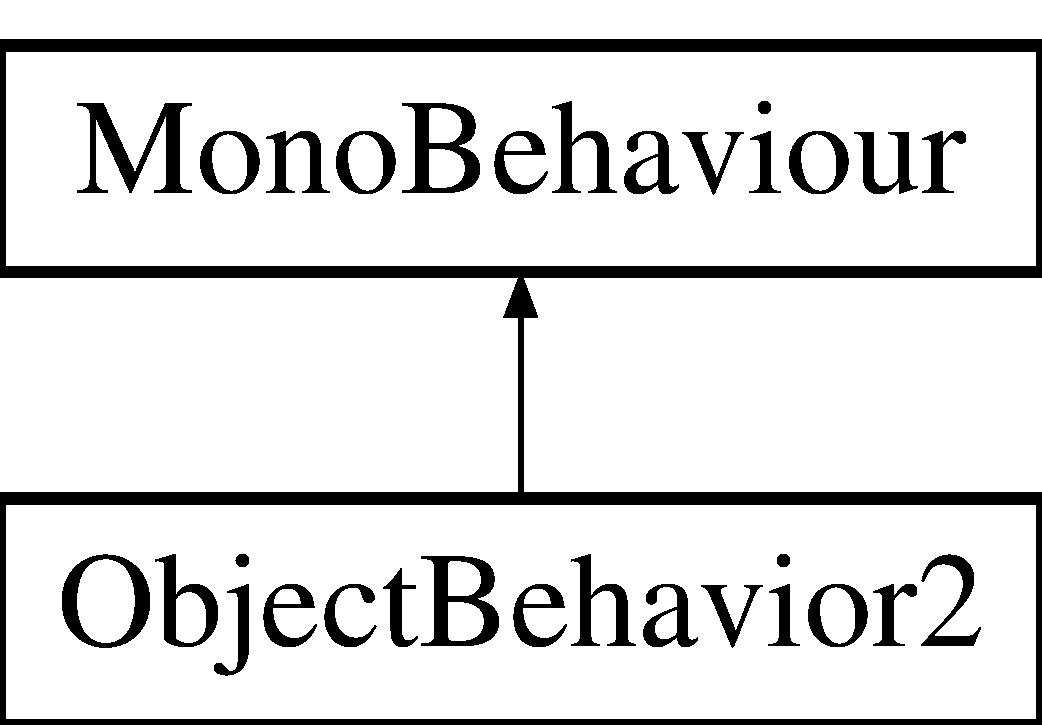
\includegraphics[height=2.000000cm]{classObjectBehavior2}
\end{center}
\end{figure}
\subsection*{Public Member Functions}
\begin{DoxyCompactItemize}
\item 
void \hyperlink{classObjectBehavior2_a825342e6f295dd91e594432c12ffbe75}{Update} ()
\begin{DoxyCompactList}\small\item\em Updates per frame. Changes position of object based on speed. Destroys object after 10 seconds. \end{DoxyCompactList}\end{DoxyCompactItemize}
\subsection*{Public Attributes}
\begin{DoxyCompactItemize}
\item 
float \hyperlink{classObjectBehavior2_a71c5a332d63c4fc276f53480f86f0641}{speed} = -\/20f
\begin{DoxyCompactList}\small\item\em The speed of Game\-Object. \end{DoxyCompactList}\end{DoxyCompactItemize}


\subsection{Member Function Documentation}
\hypertarget{classObjectBehavior2_a825342e6f295dd91e594432c12ffbe75}{\index{Object\-Behavior2@{Object\-Behavior2}!Update@{Update}}
\index{Update@{Update}!ObjectBehavior2@{Object\-Behavior2}}
\subsubsection[{Update}]{\setlength{\rightskip}{0pt plus 5cm}void Object\-Behavior2.\-Update (
\begin{DoxyParamCaption}
{}
\end{DoxyParamCaption}
)\hspace{0.3cm}{\ttfamily [inline]}}}\label{classObjectBehavior2_a825342e6f295dd91e594432c12ffbe75}


Updates per frame. Changes position of object based on speed. Destroys object after 10 seconds. 



\subsection{Member Data Documentation}
\hypertarget{classObjectBehavior2_a71c5a332d63c4fc276f53480f86f0641}{\index{Object\-Behavior2@{Object\-Behavior2}!speed@{speed}}
\index{speed@{speed}!ObjectBehavior2@{Object\-Behavior2}}
\subsubsection[{speed}]{\setlength{\rightskip}{0pt plus 5cm}float Object\-Behavior2.\-speed = -\/20f}}\label{classObjectBehavior2_a71c5a332d63c4fc276f53480f86f0641}


The speed of Game\-Object. 



The documentation for this class was generated from the following file\-:\begin{DoxyCompactItemize}
\item 
Object\-Behavior2.\-cs\end{DoxyCompactItemize}

\hypertarget{classPlayerController}{\section{Player\-Controller Class Reference}
\label{classPlayerController}\index{Player\-Controller@{Player\-Controller}}
}
Inheritance diagram for Player\-Controller\-:\begin{figure}[H]
\begin{center}
\leavevmode
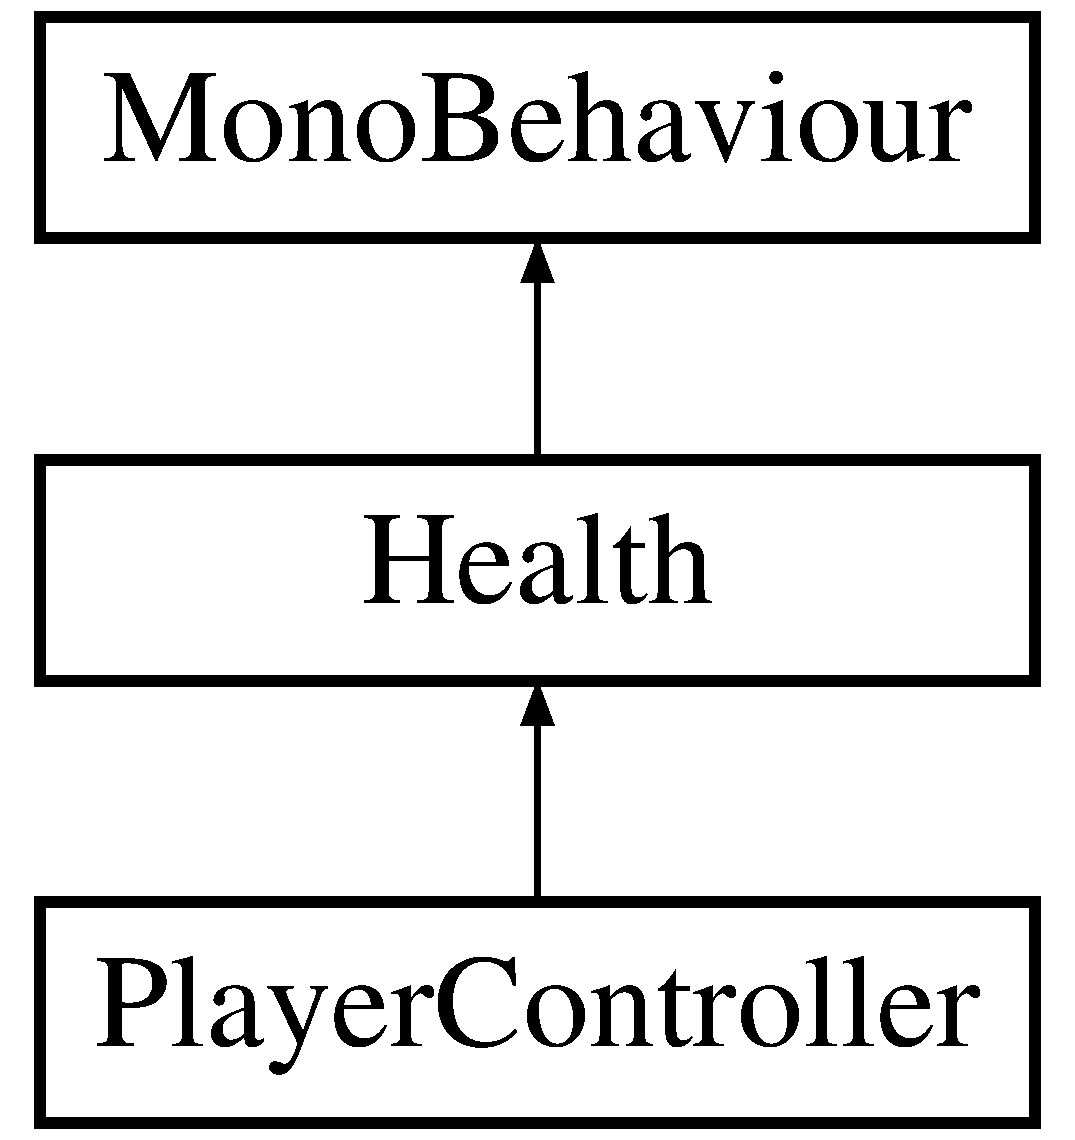
\includegraphics[height=3.000000cm]{classPlayerController}
\end{center}
\end{figure}
\subsection*{Public Member Functions}
\begin{DoxyCompactItemize}
\item 
void \hyperlink{classPlayerController_ae1117d9c4da3193181cddad2c814e467}{Start} ()
\begin{DoxyCompactList}\small\item\em Gets player physics, animator and sets audio sources to listen \end{DoxyCompactList}\item 
void \hyperlink{classPlayerController_ae8bc83dffb99867a04be016473ed2c43}{Update} ()
\begin{DoxyCompactList}\small\item\em Update per frame. check if player is dead, sets player speed, checks for user input \end{DoxyCompactList}\item 
I\-Enumerator \hyperlink{classPlayerController_a5e040cf8e9c19fc2946d979ffbd204b7}{Restart\-Level} ()
\begin{DoxyCompactList}\small\item\em Restarts the level after a 2 second delay after death. \end{DoxyCompactList}\end{DoxyCompactItemize}
\subsection*{Public Attributes}
\begin{DoxyCompactItemize}
\item 
float \hyperlink{classPlayerController_a0a8e0eb9de4ccc5bd5f4cc5b44469b01}{gravity} = 20
\begin{DoxyCompactList}\small\item\em The gravity. \end{DoxyCompactList}\item 
float \hyperlink{classPlayerController_a0928605583f0563cd84fe43119d336ec}{speed} = 8
\begin{DoxyCompactList}\small\item\em The speed. \end{DoxyCompactList}\item 
float \hyperlink{classPlayerController_a421aa51bfbc7338f353ca84ea446de96}{acceleration} = 30
\begin{DoxyCompactList}\small\item\em The acceleration. \end{DoxyCompactList}\item 
float \hyperlink{classPlayerController_a1f5dfe5afd998f509dbb405800619b6d}{jump\-Height} = 12
\begin{DoxyCompactList}\small\item\em The height of the jump. \end{DoxyCompactList}\item 
float \hyperlink{classPlayerController_a015c55d3a7c7eed11bdec88c2fb81899}{current\-Speed}
\begin{DoxyCompactList}\small\item\em The current speed. \end{DoxyCompactList}\item 
float \hyperlink{classPlayerController_a40ea46cad3dd02224b1b5d05bb530dcc}{target\-Speed}
\begin{DoxyCompactList}\small\item\em The target speed. \end{DoxyCompactList}\item 
Vector2 \hyperlink{classPlayerController_abdda9ecec7708206e6e01b1ead96f5c9}{amount\-To\-Move}
\begin{DoxyCompactList}\small\item\em The amount to move. \end{DoxyCompactList}\item 
Audio\-Source \hyperlink{classPlayerController_aa985596607cf22753896610372c00fa7}{Shot\-S\-D}
\begin{DoxyCompactList}\small\item\em The shot Sound. \end{DoxyCompactList}\item 
Audio\-Source \hyperlink{classPlayerController_a205f3898c18c6338d4e12f33222d90f5}{Roll\-S\-D}
\begin{DoxyCompactList}\small\item\em The roll Sound. \end{DoxyCompactList}\item 
Audio\-Source \hyperlink{classPlayerController_a3f516eecb6942aa1ec667de83154d350}{Jump\-S\-D}
\begin{DoxyCompactList}\small\item\em The jump Sound. \end{DoxyCompactList}\item 
Audio\-Source \hyperlink{classPlayerController_ac991ebede5b7666a4dcfefbd73114393}{Death\-S\-D}
\begin{DoxyCompactList}\small\item\em The death Sound. \end{DoxyCompactList}\item 
\hyperlink{classPlayerPhysics}{Player\-Physics} \hyperlink{classPlayerController_a039e255582f5fb656710b996fce4667e}{player\-Physics}
\begin{DoxyCompactList}\small\item\em Gets player physics script. \end{DoxyCompactList}\item 
Animator \hyperlink{classPlayerController_af6d2c371d77ff294a3840e6e26608e24}{Player}
\begin{DoxyCompactList}\small\item\em Gets player animator. \end{DoxyCompactList}\item 
float \hyperlink{classPlayerController_a499b06bd0da8f827bba77d2778814ece}{c\-Health}
\begin{DoxyCompactList}\small\item\em Variable to hold current health \end{DoxyCompactList}\item 
Game\-Object \hyperlink{classPlayerController_aabcb743694c264c111b2aa92c6f04dca}{Shot}
\begin{DoxyCompactList}\small\item\em Sets gameobject shot for prep \end{DoxyCompactList}\end{DoxyCompactItemize}


\subsection{Member Function Documentation}
\hypertarget{classPlayerController_a5e040cf8e9c19fc2946d979ffbd204b7}{\index{Player\-Controller@{Player\-Controller}!Restart\-Level@{Restart\-Level}}
\index{Restart\-Level@{Restart\-Level}!PlayerController@{Player\-Controller}}
\subsubsection[{Restart\-Level}]{\setlength{\rightskip}{0pt plus 5cm}I\-Enumerator Player\-Controller.\-Restart\-Level (
\begin{DoxyParamCaption}
{}
\end{DoxyParamCaption}
)\hspace{0.3cm}{\ttfamily [inline]}}}\label{classPlayerController_a5e040cf8e9c19fc2946d979ffbd204b7}


Restarts the level after a 2 second delay after death. 

\begin{DoxyReturn}{Returns}
The current level.
\end{DoxyReturn}
\hypertarget{classPlayerController_ae1117d9c4da3193181cddad2c814e467}{\index{Player\-Controller@{Player\-Controller}!Start@{Start}}
\index{Start@{Start}!PlayerController@{Player\-Controller}}
\subsubsection[{Start}]{\setlength{\rightskip}{0pt plus 5cm}void Player\-Controller.\-Start (
\begin{DoxyParamCaption}
{}
\end{DoxyParamCaption}
)\hspace{0.3cm}{\ttfamily [inline]}}}\label{classPlayerController_ae1117d9c4da3193181cddad2c814e467}


Gets player physics, animator and sets audio sources to listen 

\hypertarget{classPlayerController_ae8bc83dffb99867a04be016473ed2c43}{\index{Player\-Controller@{Player\-Controller}!Update@{Update}}
\index{Update@{Update}!PlayerController@{Player\-Controller}}
\subsubsection[{Update}]{\setlength{\rightskip}{0pt plus 5cm}void Player\-Controller.\-Update (
\begin{DoxyParamCaption}
{}
\end{DoxyParamCaption}
)\hspace{0.3cm}{\ttfamily [inline]}}}\label{classPlayerController_ae8bc83dffb99867a04be016473ed2c43}


Update per frame. check if player is dead, sets player speed, checks for user input 



\subsection{Member Data Documentation}
\hypertarget{classPlayerController_a421aa51bfbc7338f353ca84ea446de96}{\index{Player\-Controller@{Player\-Controller}!acceleration@{acceleration}}
\index{acceleration@{acceleration}!PlayerController@{Player\-Controller}}
\subsubsection[{acceleration}]{\setlength{\rightskip}{0pt plus 5cm}float Player\-Controller.\-acceleration = 30}}\label{classPlayerController_a421aa51bfbc7338f353ca84ea446de96}


The acceleration. 

\hypertarget{classPlayerController_abdda9ecec7708206e6e01b1ead96f5c9}{\index{Player\-Controller@{Player\-Controller}!amount\-To\-Move@{amount\-To\-Move}}
\index{amount\-To\-Move@{amount\-To\-Move}!PlayerController@{Player\-Controller}}
\subsubsection[{amount\-To\-Move}]{\setlength{\rightskip}{0pt plus 5cm}Vector2 Player\-Controller.\-amount\-To\-Move}}\label{classPlayerController_abdda9ecec7708206e6e01b1ead96f5c9}


The amount to move. 

\hypertarget{classPlayerController_a499b06bd0da8f827bba77d2778814ece}{\index{Player\-Controller@{Player\-Controller}!c\-Health@{c\-Health}}
\index{c\-Health@{c\-Health}!PlayerController@{Player\-Controller}}
\subsubsection[{c\-Health}]{\setlength{\rightskip}{0pt plus 5cm}float Player\-Controller.\-c\-Health}}\label{classPlayerController_a499b06bd0da8f827bba77d2778814ece}


Variable to hold current health 

\hypertarget{classPlayerController_a015c55d3a7c7eed11bdec88c2fb81899}{\index{Player\-Controller@{Player\-Controller}!current\-Speed@{current\-Speed}}
\index{current\-Speed@{current\-Speed}!PlayerController@{Player\-Controller}}
\subsubsection[{current\-Speed}]{\setlength{\rightskip}{0pt plus 5cm}float Player\-Controller.\-current\-Speed}}\label{classPlayerController_a015c55d3a7c7eed11bdec88c2fb81899}


The current speed. 

\hypertarget{classPlayerController_ac991ebede5b7666a4dcfefbd73114393}{\index{Player\-Controller@{Player\-Controller}!Death\-S\-D@{Death\-S\-D}}
\index{Death\-S\-D@{Death\-S\-D}!PlayerController@{Player\-Controller}}
\subsubsection[{Death\-S\-D}]{\setlength{\rightskip}{0pt plus 5cm}Audio\-Source Player\-Controller.\-Death\-S\-D}}\label{classPlayerController_ac991ebede5b7666a4dcfefbd73114393}


The death Sound. 

\hypertarget{classPlayerController_a0a8e0eb9de4ccc5bd5f4cc5b44469b01}{\index{Player\-Controller@{Player\-Controller}!gravity@{gravity}}
\index{gravity@{gravity}!PlayerController@{Player\-Controller}}
\subsubsection[{gravity}]{\setlength{\rightskip}{0pt plus 5cm}float Player\-Controller.\-gravity = 20}}\label{classPlayerController_a0a8e0eb9de4ccc5bd5f4cc5b44469b01}


The gravity. 

\hypertarget{classPlayerController_a1f5dfe5afd998f509dbb405800619b6d}{\index{Player\-Controller@{Player\-Controller}!jump\-Height@{jump\-Height}}
\index{jump\-Height@{jump\-Height}!PlayerController@{Player\-Controller}}
\subsubsection[{jump\-Height}]{\setlength{\rightskip}{0pt plus 5cm}float Player\-Controller.\-jump\-Height = 12}}\label{classPlayerController_a1f5dfe5afd998f509dbb405800619b6d}


The height of the jump. 

\hypertarget{classPlayerController_a3f516eecb6942aa1ec667de83154d350}{\index{Player\-Controller@{Player\-Controller}!Jump\-S\-D@{Jump\-S\-D}}
\index{Jump\-S\-D@{Jump\-S\-D}!PlayerController@{Player\-Controller}}
\subsubsection[{Jump\-S\-D}]{\setlength{\rightskip}{0pt plus 5cm}Audio\-Source Player\-Controller.\-Jump\-S\-D}}\label{classPlayerController_a3f516eecb6942aa1ec667de83154d350}


The jump Sound. 

\hypertarget{classPlayerController_af6d2c371d77ff294a3840e6e26608e24}{\index{Player\-Controller@{Player\-Controller}!Player@{Player}}
\index{Player@{Player}!PlayerController@{Player\-Controller}}
\subsubsection[{Player}]{\setlength{\rightskip}{0pt plus 5cm}Animator Player\-Controller.\-Player}}\label{classPlayerController_af6d2c371d77ff294a3840e6e26608e24}


Gets player animator. 

\hypertarget{classPlayerController_a039e255582f5fb656710b996fce4667e}{\index{Player\-Controller@{Player\-Controller}!player\-Physics@{player\-Physics}}
\index{player\-Physics@{player\-Physics}!PlayerController@{Player\-Controller}}
\subsubsection[{player\-Physics}]{\setlength{\rightskip}{0pt plus 5cm}{\bf Player\-Physics} Player\-Controller.\-player\-Physics}}\label{classPlayerController_a039e255582f5fb656710b996fce4667e}


Gets player physics script. 

\hypertarget{classPlayerController_a205f3898c18c6338d4e12f33222d90f5}{\index{Player\-Controller@{Player\-Controller}!Roll\-S\-D@{Roll\-S\-D}}
\index{Roll\-S\-D@{Roll\-S\-D}!PlayerController@{Player\-Controller}}
\subsubsection[{Roll\-S\-D}]{\setlength{\rightskip}{0pt plus 5cm}Audio\-Source Player\-Controller.\-Roll\-S\-D}}\label{classPlayerController_a205f3898c18c6338d4e12f33222d90f5}


The roll Sound. 

\hypertarget{classPlayerController_aabcb743694c264c111b2aa92c6f04dca}{\index{Player\-Controller@{Player\-Controller}!Shot@{Shot}}
\index{Shot@{Shot}!PlayerController@{Player\-Controller}}
\subsubsection[{Shot}]{\setlength{\rightskip}{0pt plus 5cm}Game\-Object Player\-Controller.\-Shot}}\label{classPlayerController_aabcb743694c264c111b2aa92c6f04dca}


Sets gameobject shot for prep 

\hypertarget{classPlayerController_aa985596607cf22753896610372c00fa7}{\index{Player\-Controller@{Player\-Controller}!Shot\-S\-D@{Shot\-S\-D}}
\index{Shot\-S\-D@{Shot\-S\-D}!PlayerController@{Player\-Controller}}
\subsubsection[{Shot\-S\-D}]{\setlength{\rightskip}{0pt plus 5cm}Audio\-Source Player\-Controller.\-Shot\-S\-D}}\label{classPlayerController_aa985596607cf22753896610372c00fa7}


The shot Sound. 

\hypertarget{classPlayerController_a0928605583f0563cd84fe43119d336ec}{\index{Player\-Controller@{Player\-Controller}!speed@{speed}}
\index{speed@{speed}!PlayerController@{Player\-Controller}}
\subsubsection[{speed}]{\setlength{\rightskip}{0pt plus 5cm}float Player\-Controller.\-speed = 8}}\label{classPlayerController_a0928605583f0563cd84fe43119d336ec}


The speed. 

\hypertarget{classPlayerController_a40ea46cad3dd02224b1b5d05bb530dcc}{\index{Player\-Controller@{Player\-Controller}!target\-Speed@{target\-Speed}}
\index{target\-Speed@{target\-Speed}!PlayerController@{Player\-Controller}}
\subsubsection[{target\-Speed}]{\setlength{\rightskip}{0pt plus 5cm}float Player\-Controller.\-target\-Speed}}\label{classPlayerController_a40ea46cad3dd02224b1b5d05bb530dcc}


The target speed. 



The documentation for this class was generated from the following file\-:\begin{DoxyCompactItemize}
\item 
Player\-Controller.\-cs\end{DoxyCompactItemize}

\hypertarget{classPlayerPhysics}{\section{Player\-Physics Class Reference}
\label{classPlayerPhysics}\index{Player\-Physics@{Player\-Physics}}
}
Inheritance diagram for Player\-Physics\-:\begin{figure}[H]
\begin{center}
\leavevmode
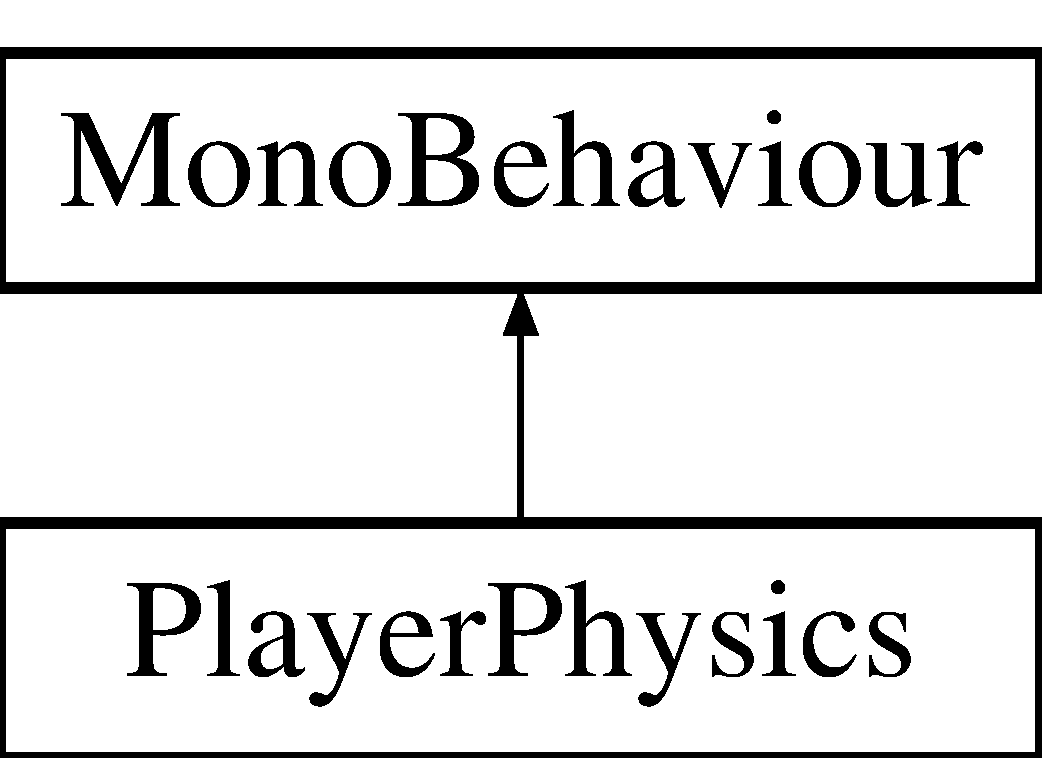
\includegraphics[height=2.000000cm]{classPlayerPhysics}
\end{center}
\end{figure}
\subsection*{Public Member Functions}
\begin{DoxyCompactItemize}
\item 
\hypertarget{classPlayerPhysics_adb50fbe957788574388514fce1dc5d89}{void {\bfseries Move} (Vector2 move\-Amount)}\label{classPlayerPhysics_adb50fbe957788574388514fce1dc5d89}

\item 
\hypertarget{classPlayerPhysics_a097b184f0e6479d3b6d58a4ac03be0a3}{void {\bfseries Set\-Collider} (Vector3 size, Vector3 centre)}\label{classPlayerPhysics_a097b184f0e6479d3b6d58a4ac03be0a3}

\item 
\hypertarget{classPlayerPhysics_a24ed69f034983045687bddc989754878}{void {\bfseries Reset\-Collider} ()}\label{classPlayerPhysics_a24ed69f034983045687bddc989754878}

\end{DoxyCompactItemize}
\subsection*{Public Attributes}
\begin{DoxyCompactItemize}
\item 
\hypertarget{classPlayerPhysics_a46b85788fa905166ae9590cac0666cf5}{Layer\-Mask {\bfseries collision\-Mask}}\label{classPlayerPhysics_a46b85788fa905166ae9590cac0666cf5}

\item 
\hypertarget{classPlayerPhysics_a4bfbf0d7e9812d79434526592790f419}{bool {\bfseries grounded}}\label{classPlayerPhysics_a4bfbf0d7e9812d79434526592790f419}

\item 
\hypertarget{classPlayerPhysics_a790c7afaa2da5eef1fe56524bc671dd4}{bool {\bfseries movement\-Stopped}}\label{classPlayerPhysics_a790c7afaa2da5eef1fe56524bc671dd4}

\end{DoxyCompactItemize}


The documentation for this class was generated from the following file\-:\begin{DoxyCompactItemize}
\item 
Player\-Physics.\-cs\end{DoxyCompactItemize}

\hypertarget{classSpikeObstacle}{\section{Spike\-Obstacle Class Reference}
\label{classSpikeObstacle}\index{Spike\-Obstacle@{Spike\-Obstacle}}
}
Inheritance diagram for Spike\-Obstacle\-:\begin{figure}[H]
\begin{center}
\leavevmode
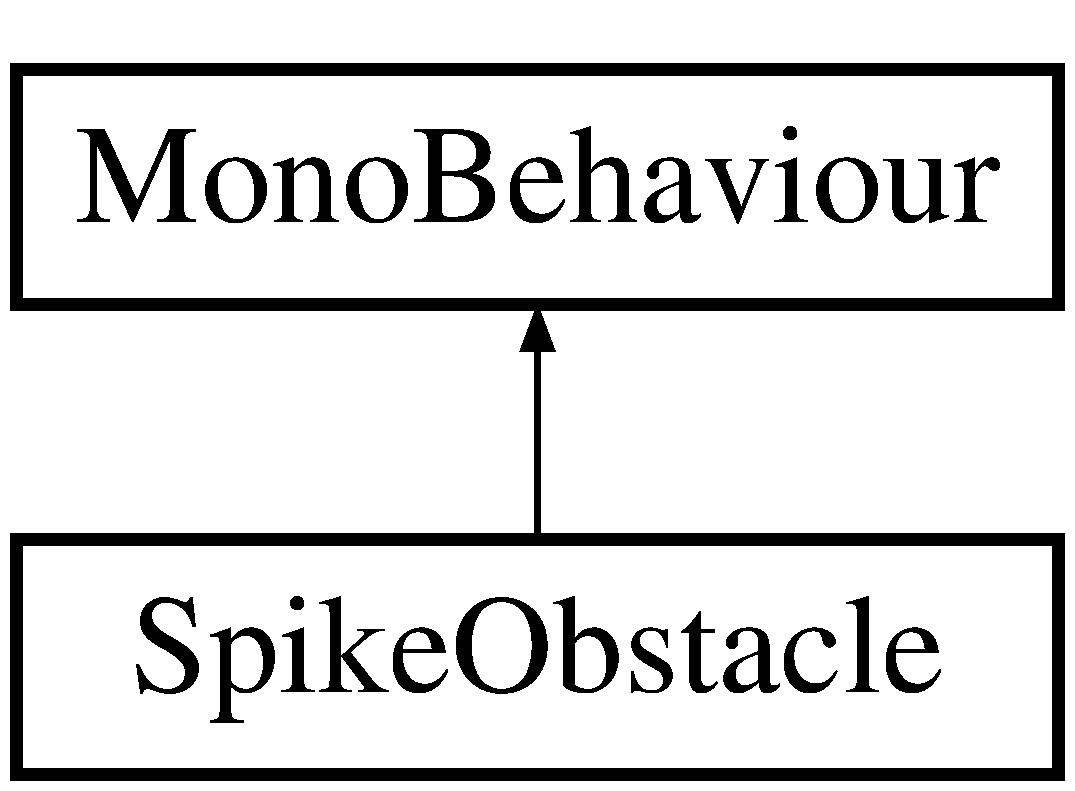
\includegraphics[height=2.000000cm]{classSpikeObstacle}
\end{center}
\end{figure}
\subsection*{Public Attributes}
\begin{DoxyCompactItemize}
\item 
\hypertarget{classSpikeObstacle_a26d288c6a9359617d93199c43e40347c}{float {\bfseries Obstacle\-Speed} = 10}\label{classSpikeObstacle_a26d288c6a9359617d93199c43e40347c}

\end{DoxyCompactItemize}


The documentation for this class was generated from the following file\-:\begin{DoxyCompactItemize}
\item 
Spike\-Obstacle.\-cs\end{DoxyCompactItemize}

\hypertarget{classTestColliderandHealth}{\section{Test\-Colliderand\-Health Class Reference}
\label{classTestColliderandHealth}\index{Test\-Colliderand\-Health@{Test\-Colliderand\-Health}}
}
Inheritance diagram for Test\-Colliderand\-Health\-:\begin{figure}[H]
\begin{center}
\leavevmode
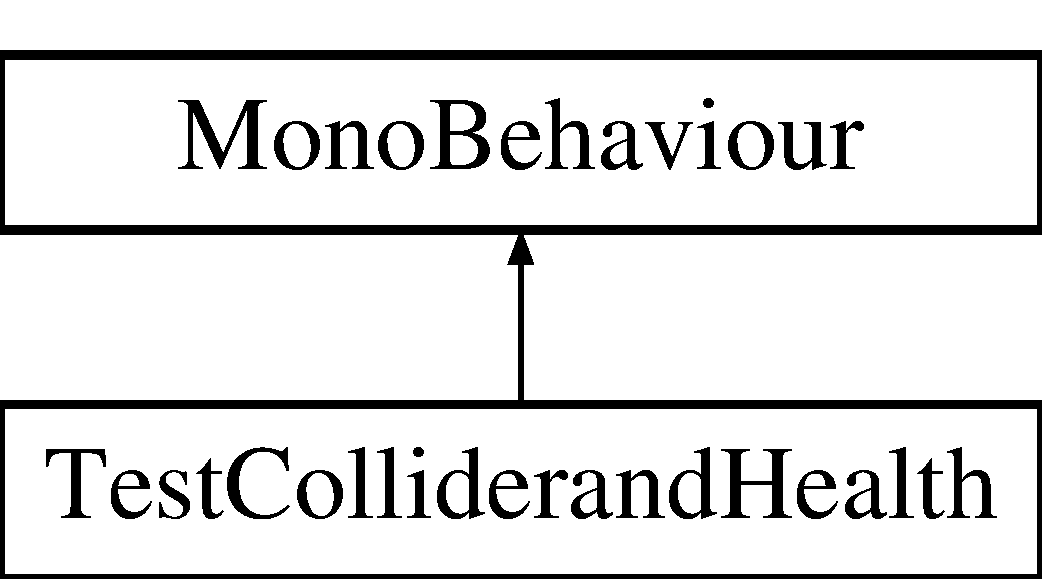
\includegraphics[height=2.000000cm]{classTestColliderandHealth}
\end{center}
\end{figure}


The documentation for this class was generated from the following file\-:\begin{DoxyCompactItemize}
\item 
Test\-Colliderand\-Health.\-cs\end{DoxyCompactItemize}

%--- End generated contents ---

% Index
\newpage
\phantomsection
\addcontentsline{toc}{chapter}{Index}
\printindex

\end{document}
